\documentclass{beamer}

\usepackage{tikz}
\usepackage{booktabs}

\usepackage{amsmath,amssymb}
\usepackage{hyperref}

\usepackage{graphicx}

\newcommand{\argmin}{\operatorname*{arg\, min}}
\newcommand{\sign}{\operatorname{sign}}
\newcommand{\RR}{\mathbb R}
\newcommand{\NN}{\mathbb N}

\DeclareMathOperator*{\maximize}{maximize}

% Set transparency of non-highlighted sections in the table of
% contents slide.
\setbeamertemplate{section in toc shaded}[default][100]
\AtBeginSection[]
{
  \setbeamercolor{section in toc}{fg=red} 
  \setbeamercolor{section in toc shaded}{fg=black} 
  \begin{frame}
    \tableofcontents[currentsection]
  \end{frame}
}

\begin{document}

\title{SegAnnDB: interactive genomic segmentation\\
\url{http://bioviz.rocq.inria.fr/}}
\newcommand{\acknowledge}[2]{\parbox{1.5in}{ \centering
\includegraphics[height=0.5in]{photos/#1}\\
#2
}}
\author{
Toby Dylan Hocking, Toby.Hocking@mail.mcgill.ca\\
\vskip 1cm
joint work with Valentina Boeva, Guillem Rigaill, Gudrun Schleiermacher, Isabelle Janoueix-Lerosey, Olivier Delattre, Wilfrid Richer, Franck Bourdeaut, Miyuki Suguro, Masao Seto, Francis Bach, and Jean-Philippe Vert.
}

%\date{12 April 2013}

\maketitle

\section{Introduction: how to detect changes in copy number?}

\begin{frame}
  \frametitle{Cancer cells show chromosomal copy number alterations}
  Spectral karyotypes show the number of copies of the sex chromosomes
  (X,Y) and autosomes (1-22). 

  Source: Alberts \emph{et al.} 2002.
\vskip 0.1in
  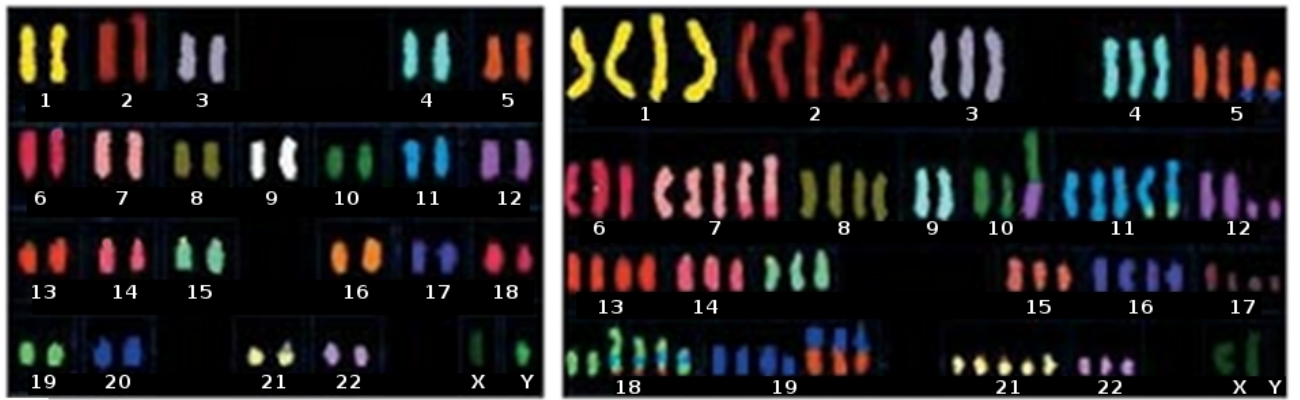
\includegraphics[width=\textwidth]{Karyo-both}
\vskip 0.1in
  \begin{minipage}{0.4\linewidth}
    Normal cell with 2 copies of each autosome.
  \end{minipage}
\hskip 0.1\linewidth
  \begin{minipage}{0.4\linewidth}
Cancer cell with many copy number alterations.
  \end{minipage}
\end{frame}

\begin{frame}
  \frametitle{Motivation: tumor genome copy number analysis}
  \begin{itemize}
  \item Comparative genomic hybridization microarrays (aCGH) allow
    genome-wide copy number analysis since logratio is proportional to
    DNA copy number (Pinkel \emph{et al.}, 1998).
  \item Tumors often contain breakpoints, amplifications, and
    deletions at specific chromosomal locations that we would like to
    detect.
  \item Which genomic alterations are linked with good or bad patient
    outcome?
  \item To answer clinical questions like this one, we first need to
    accurately detect these genomic alterations.
  \end{itemize}
\end{frame}

\begin{frame}
  \frametitle{aCGH neuroblastoma copy number data}
  
  \includegraphics[width=\textwidth]{figure-profiles}
  
\end{frame}


\begin{frame}
  \frametitle{Copy number profiles are predictive of progression in
    neuroblastoma}
  
  Gudrun Schleiermacher, \emph{et al.} Accumulation of Segmental
  Alterations Determines Progression in Neuroblastoma. J Clinical
  Oncology 2010.

  2 types of profiles:
  
  \begin{itemize}
  \item Numerical: entire chromosome amplification. \alert{Good}
    outcome.
  \item Segmental: deletion 1p 3p 11q, gain 1q 2p 17q. \alert{Bad}
    outcome. 
  \end{itemize}
  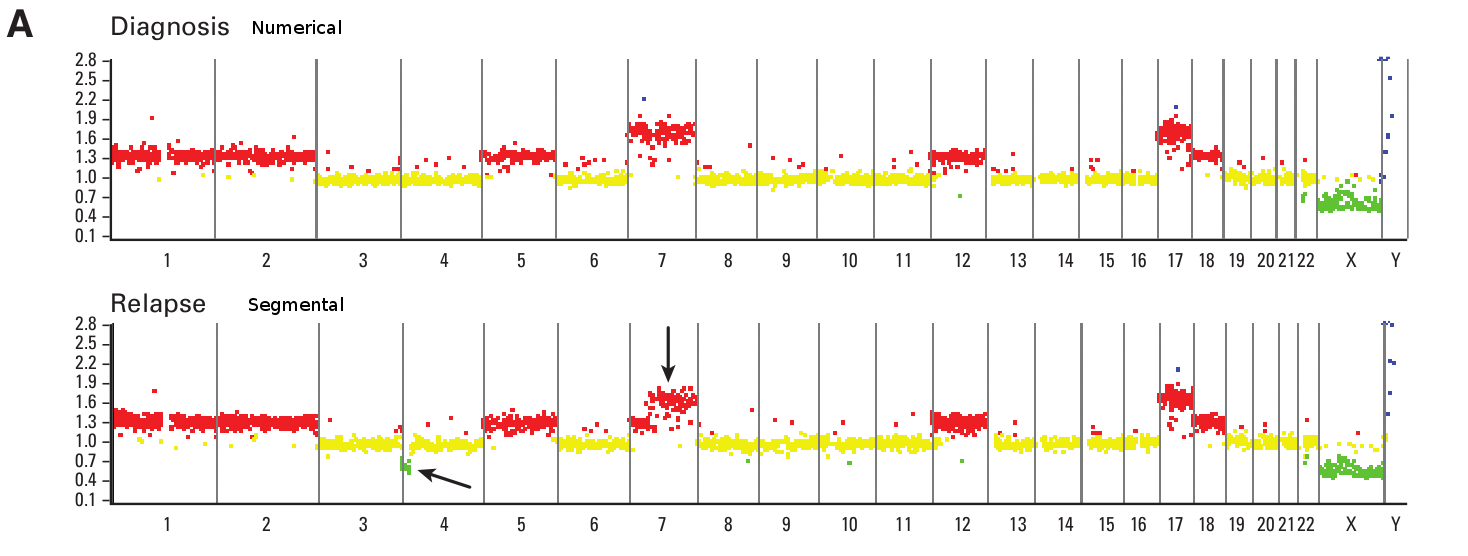
\includegraphics[width=\textwidth]{numerical-segmental}
  
\end{frame}

\section{Visual breakpoint annotations}

  \begin{frame} \frametitle{Creating breakpoint annotations (demo)}
    \includegraphics[width=\textwidth]{figure-profiles}
  \end{frame}

  \begin{frame}
    \includegraphics[width=\textwidth]{figure-annotations}
  \end{frame}

  \begin{frame}
    \includegraphics[width=\textwidth]{figure-annotations-emph}
  \end{frame}

  \begin{frame}
    \frametitle{Annotations for 2 signals}
    \input{figure-2signals}
  \end{frame}

  \begin{frame}
    \frametitle{Estimated model with 1 segment}
    \input{figure-2signals1}
  \end{frame}

  \begin{frame}
    \frametitle{Estimated model with 2 segments}
    \input{figure-2signals2}
  \end{frame}

  \begin{frame}
    \frametitle{Estimated model with 3 segments}
    \input{figure-2signals3}
  \end{frame}

  \begin{frame}
    \frametitle{Estimated model with 4 segments}
    \input{figure-2signals4}
  \end{frame}

  \begin{frame}
    \frametitle{Estimated model with 5 segments}
    \input{figure-2signals5}
  \end{frame}

  \begin{frame}
    \frametitle{Annotation error curves for 2 signals...\\which
      0-error model is best?}
    \input{figure-err-k}
  \end{frame}

  \begin{frame}
    \frametitle{Another annotated signal}
    \includegraphics[width=\textwidth]{figure-segannot}
  \end{frame}

  \begin{frame}
    \frametitle{Estimated model with 1 segment}
    \includegraphics[width=\textwidth]{figure-segannot-1}
  \end{frame}

  \begin{frame}
    \frametitle{Estimated model with 2 segments}
    \includegraphics[width=\textwidth]{figure-segannot-2}
  \end{frame}

  \begin{frame}
    \frametitle{Estimated model with 3 segments}
    \includegraphics[width=\textwidth]{figure-segannot-3}
  \end{frame}

  \begin{frame}
    \frametitle{Estimated model with 4 segments}
    \includegraphics[width=\textwidth]{figure-segannot-4}
  \end{frame}

  \begin{frame}
    \frametitle{Estimated model with 5 segments}

There are no consistent least squares models.

    \includegraphics[width=\textwidth]{figure-segannot-5}
    
     How do we find a consistent model?
  \end{frame}

\section{SegAnnDB: interactive genomic segmentation}

  \begin{frame}
    \frametitle{Problems solved by SegAnnDB}
    \begin{itemize}
    \item Statistical machine learning problems:\\
    \begin{tabular}{ccc}
      \hline
      Consistent \\
      Models & Problem & Solution \\
      \hline
      1 & none & \\
      \hline
      $>1$ & Prediction & Other annotated signals\\
      &&Hocking \emph{et al.} 2013\\
      \hline
      0 & Fitting & SegAnnot: constrained segmentation\\
      & & Hocking and Rigaill 2012\\
      \hline
    \end{tabular}
    \item Technical problems:
      \begin{itemize}
      \item \textbf{Interactive scatterplots}: zooming, annotation,
        model updates. 
      \item \textbf{Storage and data export to genome browsers}:
        probes, user-specific annotations, models.
      \end{itemize}
    \end{itemize}
  \end{frame}

  \begin{frame}
    \frametitle{Optimal prediction from limited annotations}
    \begin{itemize}
    \item \href{http://arxiv.org/abs/1004.0887}{Rigaill 2010. Pruned
        dynamic programming for optimal multiple change-point
        detection. arXiv:1004.0887.}
    $$
    \begin{aligned}
      \hat y^k = &\argmin_{\mu\in\RR^d} && ||y-\mu||^2_2\\
      &\text{such that} && \text{$\mu$ has $k-1$ changes.}
    \end{aligned}
    $$
    \item Pruned dynamic programming solver: 700 lines of C++.
    \item Python interface: 50 lines of C.
    \item Consistent models $\subseteq\{\hat y^1,\dots,\hat y^{20}\}$.
    \item Hocking et al. ICML 2013. Choose the number of segments $k$ using
      interval regression on the other annotated signals.
    \item Gradient descent solver: 100 lines of Python, run as a
      background process.
    \end{itemize}
  \end{frame}

  \begin{frame}
    \frametitle{Test error decreases as models learns from more
      labels}
    \begin{itemize}
    \item Benchmark: 3642 labeled regions across 3109 chromosomes.
    \item Train on a few chromosomes, test on the rest.
    \item Mean and SD over 60 random train set orderings.
    \end{itemize}
    % Created by tikzDevice version 0.7.0 on 2014-02-02 01:44:57
% !TEX encoding = UTF-8 Unicode
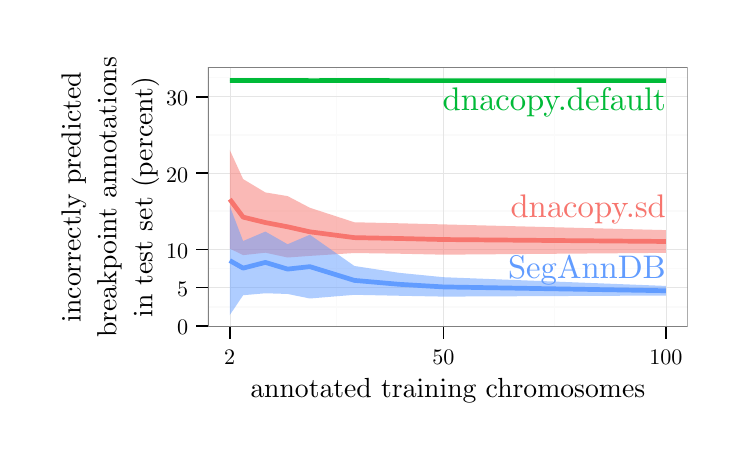
\begin{tikzpicture}[x=1pt,y=1pt]
\definecolor[named]{fillColor}{rgb}{1.00,1.00,1.00}
\path[use as bounding box,fill=fillColor,fill opacity=0.00] (0,0) rectangle (252.94,144.54);
\begin{scope}
\path[clip] (  0.00,  0.00) rectangle (252.94,144.54);
\definecolor[named]{drawColor}{rgb}{1.00,1.00,1.00}
\definecolor[named]{fillColor}{rgb}{1.00,1.00,1.00}

\path[draw=drawColor,line width= 0.6pt,line join=round,line cap=round,fill=fillColor] (  0.00,  0.00) rectangle (252.94,144.54);
\end{scope}
\begin{scope}
\path[clip] ( 65.15, 36.44) rectangle (238.49,130.09);
\definecolor[named]{fillColor}{rgb}{1.00,1.00,1.00}

\path[fill=fillColor] ( 65.15, 36.44) rectangle (238.49,130.09);
\definecolor[named]{drawColor}{rgb}{0.98,0.98,0.98}

\path[draw=drawColor,line width= 0.6pt,line join=round] ( 65.15, 43.70) --
	(238.49, 43.70);

\path[draw=drawColor,line width= 0.6pt,line join=round] ( 65.15, 57.50) --
	(238.49, 57.50);

\path[draw=drawColor,line width= 0.6pt,line join=round] ( 65.15, 78.19) --
	(238.49, 78.19);

\path[draw=drawColor,line width= 0.6pt,line join=round] ( 65.15,105.79) --
	(238.49,105.79);

\path[draw=drawColor,line width= 0.6pt,line join=round] ( 65.15,126.49) --
	(238.49,126.49);

\path[draw=drawColor,line width= 0.6pt,line join=round] (111.62, 36.44) --
	(111.62,130.09);

\path[draw=drawColor,line width= 0.6pt,line join=round] (190.41, 36.44) --
	(190.41,130.09);
\definecolor[named]{drawColor}{rgb}{0.90,0.90,0.90}

\path[draw=drawColor,line width= 0.2pt,line join=round] ( 65.15, 36.80) --
	(238.49, 36.80);

\path[draw=drawColor,line width= 0.2pt,line join=round] ( 65.15, 50.60) --
	(238.49, 50.60);

\path[draw=drawColor,line width= 0.2pt,line join=round] ( 65.15, 64.40) --
	(238.49, 64.40);

\path[draw=drawColor,line width= 0.2pt,line join=round] ( 65.15, 91.99) --
	(238.49, 91.99);

\path[draw=drawColor,line width= 0.2pt,line join=round] ( 65.15,119.59) --
	(238.49,119.59);

\path[draw=drawColor,line width= 0.2pt,line join=round] ( 73.03, 36.44) --
	( 73.03,130.09);

\path[draw=drawColor,line width= 0.2pt,line join=round] (150.21, 36.44) --
	(150.21,130.09);

\path[draw=drawColor,line width= 0.2pt,line join=round] (230.61, 36.44) --
	(230.61,130.09);
\definecolor[named]{drawColor}{rgb}{0.97,0.46,0.43}

\path[draw=drawColor,line width= 1.7pt,line join=round] ( 73.03, 82.53) --
	( 77.85, 76.08) --
	( 85.89, 74.12) --
	( 93.93, 72.58) --
	(101.97, 70.77) --
	(118.05, 68.67) --
	(134.13, 68.36) --
	(150.21, 67.98) --
	(230.61, 67.28);
\definecolor[named]{drawColor}{rgb}{0.00,0.73,0.22}

\path[draw=drawColor,line width= 1.7pt,line join=round] ( 73.03,125.46) --
	( 77.85,125.46) --
	( 85.89,125.45) --
	( 93.93,125.44) --
	(101.97,125.41) --
	(118.05,125.42) --
	(134.13,125.41) --
	(150.21,125.40) --
	(230.61,125.40);
\definecolor[named]{drawColor}{rgb}{0.38,0.61,1.00}

\path[draw=drawColor,line width= 1.7pt,line join=round] ( 73.03, 60.38) --
	( 77.85, 57.65) --
	( 85.89, 59.72) --
	( 93.93, 57.30) --
	(101.97, 58.19) --
	(118.05, 53.22) --
	(134.13, 51.81) --
	(150.21, 50.86) --
	(230.61, 49.48);
\definecolor[named]{fillColor}{rgb}{0.97,0.46,0.43}

\path[fill=fillColor,fill opacity=0.50] ( 73.03,100.34) --
	( 77.85, 89.82) --
	( 85.89, 85.00) --
	( 93.93, 83.67) --
	(101.97, 79.46) --
	(118.05, 74.22) --
	(134.13, 73.86) --
	(150.21, 73.45) --
	(230.61, 71.39) --
	(230.61, 63.17) --
	(150.21, 62.51) --
	(134.13, 62.86) --
	(118.05, 63.11) --
	(101.97, 62.07) --
	( 93.93, 61.49) --
	( 85.89, 63.23) --
	( 77.85, 62.34) --
	( 73.03, 64.73) --
	cycle;
\definecolor[named]{fillColor}{rgb}{0.00,0.73,0.22}

\path[fill=fillColor,fill opacity=0.50] ( 73.03,125.51) --
	( 77.85,125.55) --
	( 85.89,125.58) --
	( 93.93,125.60) --
	(101.97,125.58) --
	(118.05,125.64) --
	(134.13,125.67) --
	(150.21,125.70) --
	(230.61,125.83) --
	(230.61,124.96) --
	(150.21,125.10) --
	(134.13,125.15) --
	(118.05,125.20) --
	(101.97,125.25) --
	( 93.93,125.28) --
	( 85.89,125.31) --
	( 77.85,125.37) --
	( 73.03,125.41) --
	cycle;
\definecolor[named]{fillColor}{rgb}{0.38,0.61,1.00}

\path[fill=fillColor,fill opacity=0.50] ( 73.03, 80.06) --
	( 77.85, 67.44) --
	( 85.89, 70.86) --
	( 93.93, 66.28) --
	(101.97, 69.71) --
	(118.05, 58.43) --
	(134.13, 55.96) --
	(150.21, 54.37) --
	(230.61, 51.22) --
	(230.61, 47.75) --
	(150.21, 47.36) --
	(134.13, 47.67) --
	(118.05, 48.01) --
	(101.97, 46.68) --
	( 93.93, 48.32) --
	( 85.89, 48.57) --
	( 77.85, 47.86) --
	( 73.03, 40.70) --
	cycle;
\definecolor[named]{drawColor}{rgb}{0.00,0.73,0.22}

\node[text=drawColor,anchor=base east,inner sep=0pt, outer sep=0pt, scale=  1.18] at (230.61,114.71) {dnacopy.default};
\definecolor[named]{drawColor}{rgb}{0.97,0.46,0.43}

\node[text=drawColor,anchor=base east,inner sep=0pt, outer sep=0pt, scale=  1.18] at (230.61, 76.07) {dnacopy.sd};
\definecolor[named]{drawColor}{rgb}{0.38,0.61,1.00}

\node[text=drawColor,anchor=base east,inner sep=0pt, outer sep=0pt, scale=  1.18] at (230.61, 54.00) {SegAnnDB};
\definecolor[named]{drawColor}{rgb}{0.50,0.50,0.50}

\path[draw=drawColor,line width= 0.6pt,line join=round,line cap=round] ( 65.15, 36.44) rectangle (238.49,130.09);
\end{scope}
\begin{scope}
\path[clip] (  0.00,  0.00) rectangle (252.94,144.54);
\definecolor[named]{drawColor}{rgb}{0.00,0.00,0.00}

\node[text=drawColor,anchor=base east,inner sep=0pt, outer sep=0pt, scale=  0.80] at ( 58.04, 33.50) {0};

\node[text=drawColor,anchor=base east,inner sep=0pt, outer sep=0pt, scale=  0.80] at ( 58.04, 47.29) {5};

\node[text=drawColor,anchor=base east,inner sep=0pt, outer sep=0pt, scale=  0.80] at ( 58.04, 61.09) {10};

\node[text=drawColor,anchor=base east,inner sep=0pt, outer sep=0pt, scale=  0.80] at ( 58.04, 88.69) {20};

\node[text=drawColor,anchor=base east,inner sep=0pt, outer sep=0pt, scale=  0.80] at ( 58.04,116.28) {30};
\end{scope}
\begin{scope}
\path[clip] (  0.00,  0.00) rectangle (252.94,144.54);
\definecolor[named]{drawColor}{rgb}{0.00,0.00,0.00}

\path[draw=drawColor,line width= 0.6pt,line join=round] ( 60.88, 36.80) --
	( 65.15, 36.80);

\path[draw=drawColor,line width= 0.6pt,line join=round] ( 60.88, 50.60) --
	( 65.15, 50.60);

\path[draw=drawColor,line width= 0.6pt,line join=round] ( 60.88, 64.40) --
	( 65.15, 64.40);

\path[draw=drawColor,line width= 0.6pt,line join=round] ( 60.88, 91.99) --
	( 65.15, 91.99);

\path[draw=drawColor,line width= 0.6pt,line join=round] ( 60.88,119.59) --
	( 65.15,119.59);
\end{scope}
\begin{scope}
\path[clip] (  0.00,  0.00) rectangle (252.94,144.54);
\definecolor[named]{drawColor}{rgb}{0.00,0.00,0.00}

\path[draw=drawColor,line width= 0.6pt,line join=round] ( 73.03, 32.18) --
	( 73.03, 36.44);

\path[draw=drawColor,line width= 0.6pt,line join=round] (150.21, 32.18) --
	(150.21, 36.44);

\path[draw=drawColor,line width= 0.6pt,line join=round] (230.61, 32.18) --
	(230.61, 36.44);
\end{scope}
\begin{scope}
\path[clip] (  0.00,  0.00) rectangle (252.94,144.54);
\definecolor[named]{drawColor}{rgb}{0.00,0.00,0.00}

\node[text=drawColor,anchor=base,inner sep=0pt, outer sep=0pt, scale=  0.80] at ( 73.03, 22.72) {2};

\node[text=drawColor,anchor=base,inner sep=0pt, outer sep=0pt, scale=  0.80] at (150.21, 22.72) {50};

\node[text=drawColor,anchor=base,inner sep=0pt, outer sep=0pt, scale=  0.80] at (230.61, 22.72) {100};
\end{scope}
\begin{scope}
\path[clip] (  0.00,  0.00) rectangle (252.94,144.54);
\definecolor[named]{drawColor}{rgb}{0.00,0.00,0.00}

\node[text=drawColor,anchor=base,inner sep=0pt, outer sep=0pt, scale=  1.00] at (151.82, 10.84) {annotated training chromosomes};
\end{scope}
\begin{scope}
\path[clip] (  0.00,  0.00) rectangle (252.94,144.54);
\definecolor[named]{drawColor}{rgb}{0.00,0.00,0.00}

\node[text=drawColor,rotate= 90.00,anchor=base,inner sep=0pt, outer sep=0pt, scale=  1.00] at ( 19.11, 83.26) {incorrectly predicted};

\node[text=drawColor,rotate= 90.00,anchor=base,inner sep=0pt, outer sep=0pt, scale=  1.00] at ( 32.07, 83.26) {breakpoint annotations};

\node[text=drawColor,rotate= 90.00,anchor=base,inner sep=0pt, outer sep=0pt, scale=  1.00] at ( 45.03, 83.26) {in test set (percent)};
\end{scope}
\end{tikzpicture}

  \end{frame}

  \begin{frame}
    \frametitle{Optimal fitting for any annotations}
    \begin{itemize}
    \item \href{http://hal.inria.fr/hal-00759129/}{Hocking and Rigaill
        2012. SegAnnot: fast segmentation of
        annotated piecewise constant signals. HAL-00759129.}
    $$
    \begin{aligned}
      &\argmin_{\mu\in\RR^d} && ||y-\mu||^2_2\\
      &\text{such that} && \text{$\mu$ has 1 change in each
        1breakpoint region.}
    \end{aligned}
    $$
    \item Dynamic programming solver: 200 lines of C.
    \item Python interface: 100 lines of C.
    \end{itemize}
    
      Demo of optimal fitting on \url{http://bioviz.rocq.inria.fr}
  \end{frame}

  \begin{frame}
    \frametitle{Interactive zoomable scatterplots}
    \begin{itemize}
    \item On data upload, draw 5 sizes of PNG scatterplots using
      Python Imaging Library: 10Kb--1Mb for a sequence of 150,000
      points.
    \item Test your browser-dependent image size limit\\
      \url{http://sugiyama-www.cs.titech.ac.jp/~toby/images/}
    \item For a plot, first render PNG scatterplot as the background
      of an SVG element.
    \item Then ask the server for the current regions/model, and draw
      with SVG.
    \item When client changes annotations, save on server and send
      model back to client.
    \item 500 lines of Javascript/D3.
    \end{itemize}
  \end{frame}

  \begin{frame}
    \frametitle{Data storage and export}
    \begin{itemize}
    \item Web server/database: 1500 lines of Python.
    \item Berkeley DB: small fast NoSQL database.
    \item DB[key] = value, key is text, value is anything.
    \item Pyramid web framework exports data in
      \begin{itemize}
      \item JSON for plotted regions/model.
      \item bed/bedGraph for UCSC genome browser.
      \item CSV for R, etc.
      \end{itemize}
    \end{itemize}
  \end{frame}

\section{Discussion and conclusions}

\begin{frame}
  \frametitle{Discussion: SegAnnDB uses computer vision for genomic data}
  \begin{tabular}{ccc}
    Photos & Cell images & Copy number profiles \\
    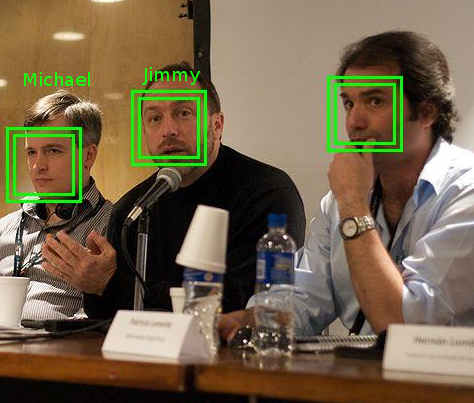
\includegraphics[width=1.3in]{faces} &
    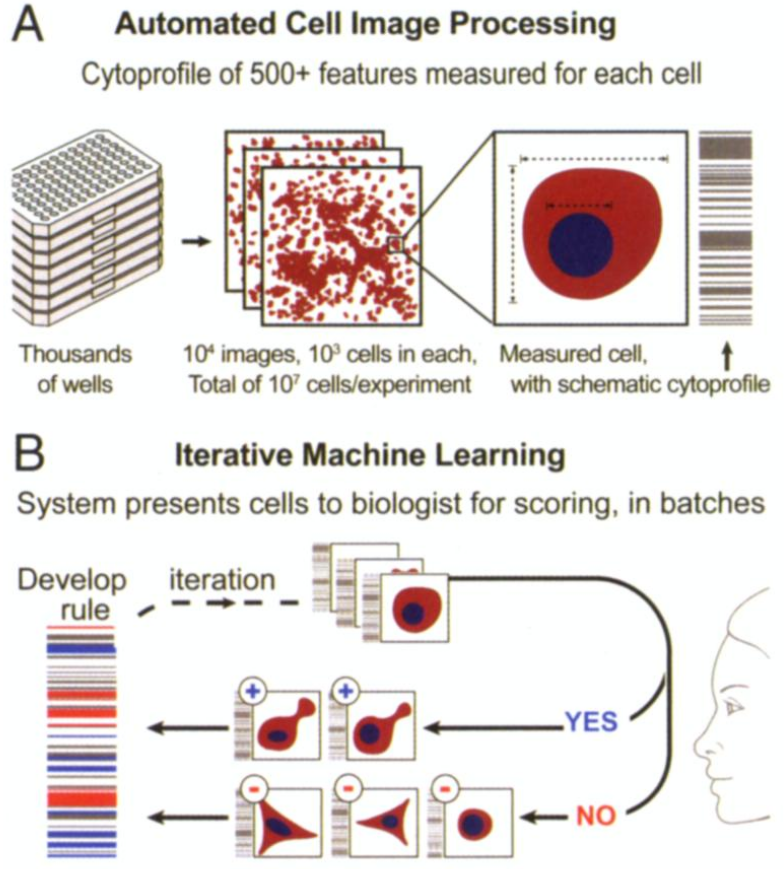
\includegraphics[width=1.3in]{cellprofiler} &
    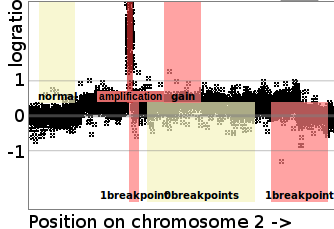
\includegraphics[width=1.5in]{regions-axes}\\
    Labels: names & phenotypes & alterations \\ \\
    CVPR 2013 & CellProfiler & SegAnnDB \\
    246 papers & 873 citations & Hocking et al, 2014. \\
    &
  \end{tabular}
  Demo: \url{http://bioviz.rocq.inria.fr}\\
  Sources: \url{http://en.wikipedia.org/wiki/Face_detection}\\
  Jones et al PNAS 2009. Scoring diverse cellular morphologies in
  image-based screens with iterative feedback and machine learning.
\end{frame}

  \begin{frame}
    \frametitle{Discussion: un-supervised versus supervised learning}
    \begin{itemize}
    \item Biologists can easily locate breakpoints and noise in plots
      of the data.
    \item \textbf{Statistics/un-supervised learning}: 
      first estimate breakpoint locations from data,
      then plot both to see if breakpoints (over- or under-)fit.
    \item \textbf{Computer vision/supervised learning}:
      first label regions with and without breakpoints, 
      then predict breakpoints that minimize the number of incorrect labels.
    \item Exploit strong points of eyes (signal/noise) and
      mathematical optimization (finding the exact breakpoint).
    \item Advantage: supervised methods more accurate.
    \item Disadvantage: need time/expertise to make labels.
    \end{itemize}    
  \end{frame}

  \begin{frame}
    \frametitle{Conclusions/availability}
    \begin{itemize}
    \item \textbf{Interactive:} SegAnnDB is the first genomic data
      analysis system with a model that is updated based on
      user-provided labels.
    \item \textbf{Accurate:} optimization algorithms are used to find
      the best model for a given set of labels.
    \item \textbf{Demo}: live on \url{http://bioviz.rocq.inria.fr/}\\
      (labeling OK, data set uploads not).
    \item \textbf{Available:} for analyzing your own data, install the
      free/open-source code on your own server/laptop:

      \url{https://github.com/tdhock/SegAnnDB}
    \end{itemize}
  \end{frame}

  \begin{frame}
    \frametitle{Help: future work}

    \begin{itemize}
    \item \textbf{Active learning}.\\
      Can we do better than random sampling?
    \item \textbf{Crowdsourcing}.\\
      If every one of you labels one profile, how do we learn a global
      model?
    \end{itemize}

    email me at Toby.Hocking@mail.mcgill.ca to collaborate!

  \end{frame}

\begin{frame}
  \frametitle{But which model is the best?}
  \begin{itemize}
  \item GLAD: adaptive weights smoothing (Hup\'e \emph{et al.}, 2004)
  \item DNAcopy: circular binary segmentation (Venkatraman and Olshen,
    2007)
  \item cghFLasso: fused lasso signal approximator with heuristics
    (Tibshirani and Wang, 2007)
  \item HaarSeg: wavelet smoothing (Ben-Yaacov and Eldar, 2008)
  \item GADA: sparse Bayesian learning (Pique-Regi \emph{et al.}, 2008)
  \item flsa: fused lasso signal approximator path algorithm (Hoefling 2009)
  \item \alert<2>{cghseg: pruned dynamic programming (Rigaill 2010)}
  \item \alert<2>{PELT: pruned exact linear time (Killick \emph{et al.}, 2011)}
  \end{itemize}
  \alert<2>{Visual annotations indicate that maximum likelihood
    segmentation is the best (Hocking \emph{et al.}, 2012).}
  \end{frame}

  \begin{frame}
    \frametitle{The cghseg.k/pelt.n least squares model}
    For a signal $y\in\RR^d$, the maximum
    likelihood model with $k\in\{1,\dots,d\}$ segments is
    $$
    \begin{aligned}
 \hat y^k=     &\argmin_{\mu\in\RR^d} && ||y-\mu||^2_2\\
      &\text{such that} && \text{$\mu$ has $k-1$ changes.}
%      &\text{subject to} && k-1 = \sum_{j=1}^{d-1}1_{\mu_{j}\neq\mu_{j+1}}
    \end{aligned}
    $$
    We select the number of segments $k$ using \textbf{visual
      annotations}.
  \end{frame}



\end{document}
